\documentclass[aspectratio=169]{beamer}

% Theme and color scheme
%\usetheme{Madrid}
 \usetheme{CambridgeUS}
\usecolortheme{seahorse}

% Packages
\usepackage{tikz}
\usepackage{pgfplots}
\pgfplotsset{compat=1.18}
\usepackage{listings}
\usepackage{xcolor}
\usepackage{fontawesome5}
\usepackage{multicol}

\usepackage[utf8]{inputenc}
\usepackage{newunicodechar}
\newunicodechar{❌}{\textcolor{red}{$\times$}}
\newunicodechar{✅}{\textcolor{green}{$\checkmark$}}
\newunicodechar{📧}{\textcolor{blue}{\faEnvelope}}
\newunicodechar{🔗}{\textcolor{blue}{\faLink}}


% Logo setup
\titlegraphic{
\includegraphics[width=3cm]{genius_sports_logo.png}}

% Custom colors
\definecolor{geniusblue}{RGB}{0,102,204}
\definecolor{darkgray}{RGB}{64,64,64}
\definecolor{lightgray}{RGB}{240,240,240}
\definecolor{alertred}{RGB}{204,0,51}
\definecolor{successgreen}{RGB}{0,153,76}

% Code listing style
\lstdefinestyle{gostyle}{
    language=Go,
    basicstyle=\tiny\ttfamily,
    keywordstyle=\color{blue}\bfseries,
    commentstyle=\color{gray},
    stringstyle=\color{red},
    numberstyle=\tiny\color{gray},
    breaklines=true,
    frame=single,
    backgroundcolor=\color{lightgray},
    showstringspaces=false,
    tabsize=2
}

 \pgfdeclareimage[height=0.5cm]{logo}{GENIUS_SPORTS_HORIZONTAL_SMALL_WHITE_RGB}
    \logo{\pgfuseimage{logo}}

% Title page information
\title[Circuit Breakers]{Circuit Breakers in Distributed Systems}
\subtitle{Building Resilient Microservices}
\author{SMA - Sports Models APIs Team}
\institute{Genius Sports}
\date{June 6, 2025}

% Custom commands
\newcommand{\circuitopen}{\textcolor{red}{\faTimesCircle}}
\newcommand{\circuitclosed}{\textcolor{green}{\faCheckCircle}}
\newcommand{\circuithalf}{\textcolor{orange}{\faAdjust}}
\newcommand{\alertred}[1]{\textcolor{red}{#1}}
\newcommand{\successgreen}[1]{\textcolor{green}{#1}}

\begin{document}

% Title slide
\begin{frame}
    \titlepage
\end{frame}

% Table of contents
\begin{frame}{Agenda}
    \tableofcontents
\end{frame}

\section{Introduction}

\begin{frame}{What We'll Cover Today}
    \begin{columns}
        \begin{column}{0.5\textwidth}
            \begin{itemize}
                \item \textbf{The Problem:} System overload can cvause
                      failures in distributed architectures
                \item \textbf{The Solution/Mitigation:} Circuit breaker pattern
                \item \textbf{The Analogy:} How electrical circuits protect systems
                \item \textbf{The Implementation:} Our Go-based circuit breaker
                \item \textbf{The Practice:} Real-world usage and monitoring
                \item \textbf{The Future:} Planned enhancements
            \end{itemize}
        \end{column}
        \begin{column}{0.5\textwidth}
            \begin{center}
                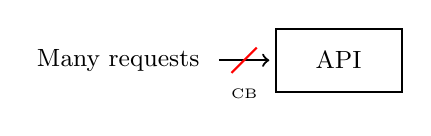
\begin{tikzpicture}[scale=0.8]
                 % Simple system diagram
                 \node at (0.5,0.5) {\small Many requests};
                    
                 \draw[thick] (3,0) rectangle (5,1);
                 \node at (4,0.5) {\small API};
                    
                 \draw[thick,->] (2.1,0.5) -- (2.9,0.5);
                    
                 % Circuit breaker symbol
                 \draw[thick,red] (2.3,0.3) -- (2.7,0.7);
                 \node[below] at (2.5,0.2) {\tiny CB};
                \end{tikzpicture}
            \end{center}
        \end{column}
    \end{columns}
\end{frame}

\section{The Problem}

\begin{frame}{Cascading Failures in Distributed Systems}
    \begin{columns}
        \begin{column}{0.7\textwidth}
            \textbf{Common Scenario: something weird affects latency of a $\mu$-service}
            
            \vspace{0.3cm}
            \textbf{Little's Law Impact:}
            \begin{itemize}
                \item \textcolor{geniusblue}{$L = \lambda × W$} (Requests in system = Arrival rate × Wait time)
                \item Higher latency \textbf{W} → More requests stuck in system \textbf{L}
                \item Increased memory consumption from queued requests
                \item Resource exhaustion accelerates
            \end{itemize}
            
            \vspace{0.3cm}
            \textbf{Without Protection:}
            \begin{itemize}
                \item[\alertred{\faTimes}] Threads get blocked waiting
                \item[\alertred{\faTimes}] Memory pressure increases
                \item[\alertred{\faTimes}] System becomes unresponsive
                \item[\alertred{\faTimes}] Cascade failure propagates
            \end{itemize}
        \end{column}
     \hspace{-0.25\textwidth}
        \begin{column}{0.4\textwidth}
            \begin{center}
                \textbf{Failure Propagation}
                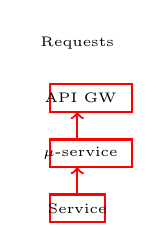
\begin{tikzpicture}[scale=0.7]
                    % Requests
                    %\draw[thick] (0,4) rectangle (1,4.5);
                    \node at (0.5,4.25) {\tiny Requests};
                    
                    % API Gateway
                    \draw[thick,red] (0,3) rectangle (1.5,3.5);
                    \node at (0.5,3.25) {\tiny \ API GW};
                    
                    % Service
                    \draw[thick,red] (0,2) rectangle (1.5,2.5);
                    \node at (0.5,2.25) {\tiny $\ \mu$-service};
                    
                    % Service
                    \draw[thick,red] (0,1) rectangle (1,1.5);
                    \node at (0.5,1.25) {\tiny Service};
                    
                    % Arrows showing failure propagation
                    \draw[thick,red,->] (0.5,1.5) -- (0.5,2);
                    \draw[thick,red,->] (0.5,2.5) -- (0.5,3);
                \end{tikzpicture}
                
                \vspace{0.4cm}                
                \textbf{Little's Law Effect}
                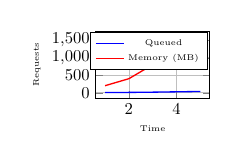
\begin{tikzpicture}[scale=0.6]
                    \begin{axis}[
                        width=4cm,
                        height=3cm,
                        xlabel={\tiny Time},
                        ylabel={\tiny Requests},
                        grid=major,
                        legend style={font=\tiny}
                    ]
                    \addplot[blue,thick] coordinates {
                        (1,5) (2,8) (3,15) (4,25) (5,35)
                    };
                    \addlegendentry{Queued}
                    
                    \addplot[red,thick] coordinates {
                        (1,200) (2,400) (3,800) (4,1200) (5,1600)
                    };
                    \addlegendentry{Memory (MB)}
                    \end{axis}
                \end{tikzpicture}
            \end{center}
        \end{column}
    \end{columns}
\end{frame}

\section{The Electrical Circuit Analogy}

\begin{frame}{How Electrical Circuit Breakers Work}
    \begin{columns}
        \begin{column}{0.5\textwidth}
            \textbf{Electrical Circuit Breaker:}
            \begin{itemize}
                \item Monitors electrical current
                \item Detects overcurrent conditions
                \item Automatically disconnects circuit
                \item Prevents fire and equipment damage
                \item Can be manually reset
            \end{itemize}
            
            \vspace{0.5cm}
            \textbf{Three States:}
            \begin{itemize}
                \item[\circuitclosed] \textbf{Closed:} Normal operation
                \item[\circuitopen] \textbf{Open:} Circuit disconnected
                \item[\circuithalf] \textbf{Half-Open:} Testing recovery
            \end{itemize}
        \end{column}
        \begin{column}{0.5\textwidth}
            \begin{center}
                \textbf{Electrical Circuit}
                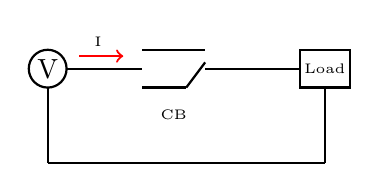
\begin{tikzpicture}[scale=0.8]
                    % Power source
                    \draw[thick] (0,1) circle (0.3);
                    \node at (0,1) {V};
                    
                    % Circuit breaker (closed)
                    \draw[thick] (1.5,1.3) -- (2.5,1.3);
                    \draw[thick] (1.5,0.7) -- (2.2,0.7);
                    \draw[thick] (2.2,0.7) -- (2.5,1.1);
                    \node[below] at (2,0.5) {\tiny CB};
                    
                    % Load
                    \draw[thick] (4,0.7) rectangle (4.8,1.3);
                    \node at (4.4,1) {\tiny Load};
                    
                    % Wires
                    \draw[thick] (0.3,1) -- (1.5,1);
                    \draw[thick] (2.5,1) -- (4,1);
                    \draw[thick] (0,-0.5) -- (4.4,-0.5);
                    \draw[thick] (0,0.7) -- (0,-0.5);
                    \draw[thick] (4.4,0.7) -- (4.4,-0.5);
                    
                    % Current flow
                    \draw[->,red,thick] (0.5,1.2) -- (1.2,1.2);
                    \node[above] at (0.8,1.2) {\tiny I};
                \end{tikzpicture}
                
                \vspace{0.5cm}
                
                \textbf{When Overloaded}
                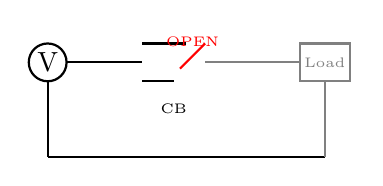
\begin{tikzpicture}[scale=0.8]
                    % Same as above but breaker open
                    \draw[thick] (0,1) circle (0.3);
                    \node at (0,1) {V};
                    
                    % Circuit breaker (open)
                    \draw[thick] (1.5,1.3) -- (2.2,1.3);
                    \draw[thick] (1.5,0.7) -- (2.0,0.7);
                    \draw[thick,red] (2.1,0.9) -- (2.5,1.3);
                    \node[below] at (2,0.5) {\tiny CB};
                    \node[above,red] at (2.3,1.1) {\tiny OPEN};
                    
                    % Load (no power)
                    \draw[thick,gray] (4,0.7) rectangle (4.8,1.3);
                    \node[gray] at (4.4,1) {\tiny Load};
                    
                    % Wires
                    \draw[thick] (0.3,1) -- (1.5,1);
                    \draw[thick,gray] (2.5,1) -- (4,1);
                    \draw[thick] (0,-0.5) -- (4.4,-0.5);
                    \draw[thick] (0,0.7) -- (0,-0.5);
                    \draw[thick,gray] (4.4,0.7) -- (4.4,-0.5);
                \end{tikzpicture}
            \end{center}
        \end{column}
    \end{columns}
\end{frame}

\begin{frame}{Software Circuit Breaker Analogy}
    \begin{center}
        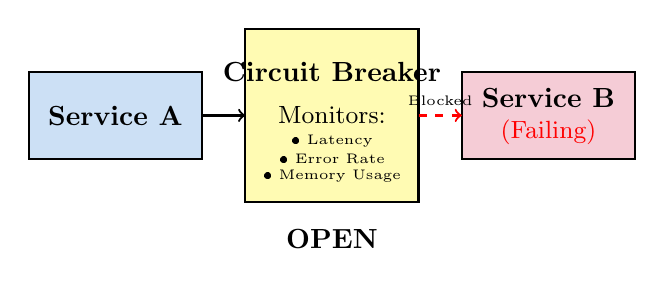
\begin{tikzpicture}[scale=1.1]
            % Service A
            \draw[thick,fill=geniusblue!20] (0,1) rectangle (2,2);
            \node at (1,1.5) {\textbf{Service A}};
            
            % Circuit Breaker
            \draw[thick,fill=yellow!30] (2.5,0.5) rectangle (4.5,2.5);
            \node at (3.5,2) {\textbf{Circuit Breaker}};
            \node at (3.5,1.5) {\small Monitors:};
            \node at (3.5,1.2) {\tiny • Latency};
            \node at (3.5,1.0) {\tiny • Error Rate};
            \node at (3.5,0.8) {\tiny • Memory Usage};
            
            % Service B
            \draw[thick,fill=alertred!20] (5,1) rectangle (7,2);
            \node at (6,1.7) {\textbf{Service B}};
            \node[red] at (6,1.3) {\small (Failing)};
            
            % Arrows
            \draw[thick,->] (2,1.5) -- (2.5,1.5);
            \draw[thick,->,red,dashed] (4.5,1.5) -- (5,1.5);
            \node[above] at (4.75,1.5) {\tiny Blocked};
            
            % Status indicators
            \node[below] at (3.5,0.3) {\circuitopen \textbf{OPEN}};
        \end{tikzpicture}
    \end{center}
    
    \begin{columns}
        \begin{column}{0.5\textwidth}
            \textbf{Software Equivalent:}
            \begin{itemize}
                \item Monitors \textbf{latency}, \textbf{errors}, \textbf{memory}
                \item Detects degraded service conditions
                \item Blocks requests to failing service
                \item Provides fallback responses
                \item Automatically attempts recovery
            \end{itemize}
        \end{column}
        \begin{column}{0.5\textwidth}
            \textbf{Benefits:}
            \begin{itemize}
                \item[\successgreen{\faCheck}] Prevents cascade failures
                \item[\successgreen{\faCheck}] Reduces resource exhaustion
                \item[\successgreen{\faCheck}] Faster failure detection
                \item[\successgreen{\faCheck}] Graceful degradation
                \item[\successgreen{\faCheck}] System stability
            \end{itemize}
        \end{column}
    \end{columns}
\end{frame}

\section{Circuit Breaker States}

\begin{frame}{Our Current Implementation: Two States}
    \begin{center}
        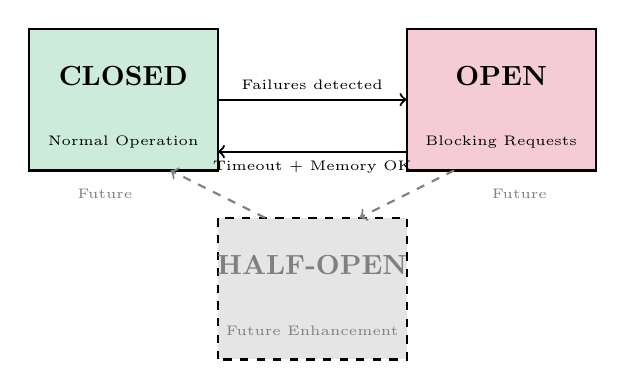
\begin{tikzpicture}[scale=1.2]
            % Closed State
            \draw[thick,fill=successgreen!20] (-2,2) rectangle (0,3.5);
            \node at (-1,3) {\textbf{CLOSED}};
            \node at (-1,2.7) {\circuitclosed};
            \node at (-1,2.3) {\tiny Normal Operation};
            
            % Open State
            \draw[thick,fill=alertred!20] (2,2) rectangle (4,3.5);
            \node at (3,3) {\textbf{OPEN}};
            \node at (3,2.7) {\circuitopen};
            \node at (3,2.3) {\tiny Blocking Requests};
            
            % Half-Open State (Future)
            \draw[thick,fill=gray!20,dashed] (0,0) rectangle (2,1.5);
            \node[gray] at (1,1) {\textbf{HALF-OPEN}};
            \node[gray] at (1,0.7) {\circuithalf};
            \node[gray] at (1,0.3) {\tiny Future Enhancement};
            
            % Transitions
            \draw[thick,->] (0,2.75) -- (2,2.75);
            \node[above] at (1,2.75) {\tiny Failures detected};
            
            \draw[thick,->] (2,2.2) -- (0,2.2);
            \node[below] at (1,2.2) {\tiny Timeout + Memory OK};
            
            % Future transition (dashed)
            \draw[thick,->,dashed,gray] (2.5,2) -- (1.5,1.5);
            \node[right,gray] at (2.8,1.75) {\tiny Future};
            
            \draw[thick,->,dashed,gray] (0.5,1.5) -- (-0.5,2);
            \node[left,gray] at (-0.8,1.75) {\tiny Future};
        \end{tikzpicture}
    \end{center}
    
    \begin{columns}
        \begin{column}{0.5\textwidth}
            \textbf{CLOSED} \circuitclosed
            \begin{itemize}
                \item Normal operation
                \item All requests pass through
                \item Monitoring metrics
                \item Ready to trip on failures
            \end{itemize}
            
            \textbf{OPEN} \circuitopen
            \begin{itemize}
                \item Blocking all requests
                \item Fast-fail responses
                \item Waiting for recovery timeout
                \item Direct transition to CLOSED
            \end{itemize}
        \end{column}
        \begin{column}{0.5\textwidth}
            \textbf{Current Limitation:}
            \begin{itemize}
                \item[\alertred{\faTimes}] No gradual recovery testing
                \item[\alertred{\faTimes}] Abrupt state transitions
                \item[\alertred{\faTimes}] No limited request probing
            \end{itemize}
            
            \textbf{Recovery Logic:}
            \begin{itemize}
                \item Wait for configured timeout
                \item Check memory status is OK
                \item Immediately transition to CLOSED
                \item Start allowing all requests
            \end{itemize}
        \end{column}
    \end{columns}
\end{frame}

\section{Our Implementation}

\begin{frame}{Go Circuit Breaker Architecture}
    \begin{center}
        \textbf{Component Overview}
        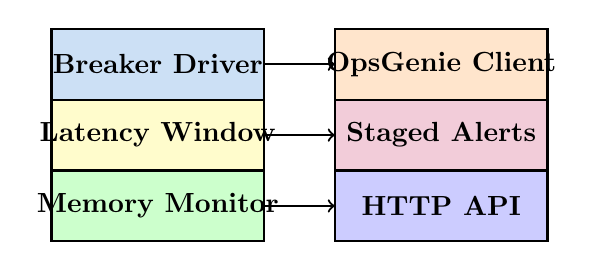
\begin{tikzpicture}[scale=0.9]
            % Main components
            \draw[thick,fill=geniusblue!20] (0,3) rectangle (3,4);
            \node at (1.5,3.5) {\textbf{Breaker Driver}};
            
            \draw[thick,fill=yellow!20] (0,2) rectangle (3,3);
            \node at (1.5,2.5) {\textbf{Latency Window}};
            
            \draw[thick,fill=green!20] (0,1) rectangle (3,2);
            \node at (1.5,1.5) {\textbf{Memory Monitor}};
            
            \draw[thick,fill=orange!20] (4,3) rectangle (7,4);
            \node at (5.5,3.5) {\textbf{OpsGenie Client}};
            
            \draw[thick,fill=purple!20] (4,2) rectangle (7,3);
            \node at (5.5,2.5) {\textbf{Staged Alerts}};
            
            \draw[thick,fill=blue!20] (4,1) rectangle (7,2);
            \node at (5.5,1.5) {\textbf{HTTP API}};
            
            % Connections
            \draw[thick,->] (3,3.5) -- (4,3.5);
            \draw[thick,->] (3,2.5) -- (4,2.5);
            \draw[thick,->] (3,1.5) -- (4,1.5);
        \end{tikzpicture}
    \end{center}
    
    \textbf{Key Features:}
    \begin{multicols}{2}
        \begin{itemize}
            \item Memory usage monitoring
            \item Latency percentile tracking
            \item Trend analysis
            \item OpsGenie integration
            \item Staged alerting system
            \item HTTP management API
            \item TOML configuration
            \item Thread-safe operations
        \end{itemize}
    \end{multicols}
\end{frame}

\begin{frame}[fragile]{Configuration Example}
\begin{lstlisting}[style=gostyle]
# Circuit Breaker Configuration
memory_threshold = 80.0              # 80% memory limit
latency_threshold = 1500             # 1500ms threshold
latency_window_size = 64             # Track last 64 operations
percentile = 0.95                    # 95th percentile
wait_time = 10                       # Wait 10 seconds before reset
trend_analysis_enabled = true        # Enable trend detection

[opsgenie]
enabled = true
region = "us"
priority = "P2"
team = "Sports Models APIs"
environment = "production"

# Alert triggers
trigger_on_breaker_open = true
trigger_on_memory_threshold = true
trigger_on_latency_threshold = true

# Staged alerting
time_before_send_alert = 60          # Escalate after 60 seconds
initial_alert_priority = "P3"        # Low priority initially
escalated_alert_priority = "P1"      # High priority if persists
\end{lstlisting}
\end{frame}

\begin{frame}[fragile]{Basic Usage}
\begin{lstlisting}[style=gostyle]
// Create breaker from configuration
breaker, err := breaker.NewBreakerFromConfigFile("config.toml")

// In any request handler
func handleRequest(w http.ResponseWriter, r *http.Request) {
    // Check if circuit breaker allows the request
    if !breaker.Allow() {
        http.Error(w, "API throttling", 429)
        return
    }
    
    startTime := time.Now()
    
    // Call your downstream service
    response, err := callDownstreamService()
    
    endTime := time.Now()
    
    // Report the latency to the circuit breaker
    breaker.Done(startTime, endTime)
    
    if err != nil {
        http.Error(w, err.Error(), 500)
        return
    }
    
    w.Write(response)
}
\end{lstlisting}
\end{frame}

\section{Advanced Features}

\begin{frame}{Trend Analysis}
    \begin{columns}
        \begin{column}{0.5\textwidth}
            \textbf{Why Trend Analysis?}
            \begin{itemize}
                \item Not all high latencies indicate problems
                \item Temporary spikes vs sustained degradation
                \item Reduces false positives
                \item Smarter triggering decisions
            \end{itemize}
            
            \vspace{0.3cm}
            \textbf{How it works:}
            \begin{itemize}
                \item Analyzes latency patterns over time
                \item Uses linear regression
                \item Detects positive trends
                \item Combines with threshold checks
            \end{itemize}
        \end{column}
        \begin{column}{0.5\textwidth}
            \begin{center}
                \textbf{Latency Patterns}
                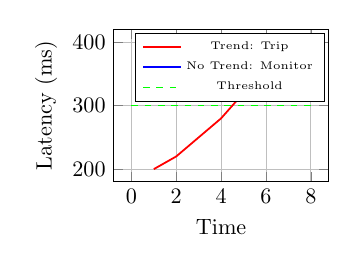
\begin{tikzpicture}[scale=0.8]
                    \begin{axis}[
                        width=5cm,
                        height=4cm,
                        xlabel=Time,
                        ylabel=Latency (ms),
                        legend style={font=\tiny},
                        grid=major
                    ]
                    \addplot[red,thick] coordinates {
                        (1,200) (2,220) (3,250) (4,280) (5,320) (6,360) (7,400)
                    };
                    \addlegendentry{Trend: Trip}
                    
                    \addplot[blue,thick] coordinates {
                        (1,350) (2,320) (3,340) (4,330) (5,345) (6,335) (7,340)
                    };
                    \addlegendentry{No Trend: Monitor}
                    
                    \addplot[green,dashed] coordinates {
                        (0,300) (8,300)
                    };
                    \addlegendentry{Threshold}
                    \end{axis}
                \end{tikzpicture}
            \end{center}
        \end{column}
    \end{columns}
\end{frame}

\begin{frame}{Staged Alerting System}
    \begin{center}
        \textbf{Progressive Alert Escalation}
        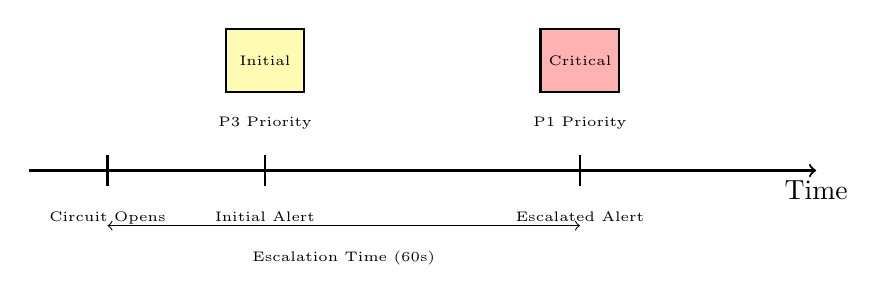
\begin{tikzpicture}[scale=1.0]
            % Timeline
            \draw[thick,->] (0,1) -- (10,1);
            \node[below] at (10,1) {Time};
            
            % Events
            \draw[thick] (1,0.8) -- (1,1.2);
            \node[below] at (1,0.6) {\tiny Circuit Opens};
            
            \draw[thick] (3,0.8) -- (3,1.2);
            \node[below] at (3,0.6) {\tiny Initial Alert};
            \node[above] at (3,1.4) {\tiny P3 Priority};
            
            \draw[thick] (7,0.8) -- (7,1.2);
            \node[below] at (7,0.6) {\tiny Escalated Alert};
            \node[above] at (7,1.4) {\tiny P1 Priority};
            
            % Alert boxes
            \draw[thick,fill=yellow!30] (2.5,2) rectangle (3.5,2.8);
            \node at (3,2.4) {\tiny Initial};
            
            \draw[thick,fill=red!30] (6.5,2) rectangle (7.5,2.8);
            \node at (7,2.4) {\tiny Critical};
            
            % Duration indicators
            \draw[<->] (1,0.3) -- (7,0.3);
            \node[below] at (4,0.1) {\tiny Escalation Time (60s)};
        \end{tikzpicture}
    \end{center}
    
    \begin{columns}
        \begin{column}{0.5\textwidth}
            \textbf{Benefits:}
            \begin{itemize}
                \item Reduces alert fatigue
                \item Appropriate response urgency
                \item Context about issue duration
                \item Automatic resolution tracking
            \end{itemize}
        \end{column}
     
     \hspace{-0.5cm}
        \begin{column}{0.55\textwidth}
            \textbf{Flow:}
            \begin{enumerate}
                \item Circuit breaker opens
                \item Send alert P3
                \item Monitor for recovery
                \item If still failing after timeout $\Rightarrow$ send alert P1
                \item Auto-resolve when recovered
            \end{enumerate}
        \end{column}
    \end{columns}
\end{frame}

\begin{frame}{Memory Monitoring}
    \begin{columns}
        \begin{column}{0.5\textwidth}
            \textbf{Why Monitor Memory?}
            \begin{itemize}
                \item Memory pressure causes GC thrashing
                \item Performance degrades before OOM
                \item Early warning system
                \item Kubernetes-aware limits
             \item Avoids OOM kills
            \end{itemize}
            
            \vspace{0.3cm}
            \textbf{Implementation:}
            \begin{itemize}
                \item Reads cgroup memory limits
                \item Monitors actual usage
                \item Configurable thresholds
                \item Integrates with circuit logic
            \end{itemize}
        \end{column}
        \begin{column}{0.5\textwidth}
            \begin{center}
                \textbf{Memory Usage Pattern}
                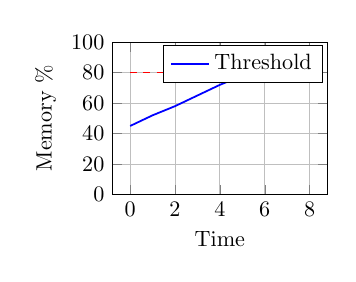
\begin{tikzpicture}[scale=0.8]
                    \begin{axis}[
                        width=5cm,
                        height=4cm,
                        xlabel=Time,
                        ylabel=Memory \%,
                        ymin=0,
                        ymax=100,
                        grid=major
                    ]
                    \addplot[blue,thick] coordinates {
                        (0,45) (1,52) (2,58) (3,65) (4,72) (5,78) (6,85) (7,92)
                    };
                    
                    \addplot[red,dashed] coordinates {
                        (0,80) (8,80)
                    };
                    \addlegendentry{Threshold}
                    
                    % Trigger point
                    \addplot[red,only marks,mark=*,mark size=3] coordinates {(6,85)};
                    \node[above] at (6,85) {\tiny Trip};
                    \end{axis}
                \end{tikzpicture}
            \end{center}
        \end{column}
    \end{columns}
\end{frame}

\section{Real-World Usage}

\begin{frame}{Circuit Breaker Integration in Montecarlo APIs}
    \begin{center}
        \begin{itemize}
         \item Basketball NBA
         \item Baseball FIBA
         \item American Football NFL
              
        \end{itemize}
    \end{center}
    
    \textbf{Protection Points: Gateways}
\end{frame}

\begin{frame}{Monitoring and Alerting}
    \begin{columns}
        \begin{column}{0.5\textwidth}
            \textbf{HTTP Management API:}
            \begin{itemize}
                \item \texttt{GET /breaker/status}
                \item \texttt{POST /breaker/reset}
                \item \texttt{GET /breaker/memory}
                \item \texttt{GET /breaker/latency}
                \item \texttt{POST /breaker/opsgenie/toggle}
            \end{itemize}
            
            \vspace{0.3cm}
            \textbf{OpsGenie Integration:}
            \begin{itemize}
                \item Automatic alert creation
                \item Rich context and metrics
                \item Team routing
                \item Alert cooldowns
            \end{itemize}
        \end{column}
        \begin{column}{0.5\textwidth}
            \textbf{Sample Alert:}
            \begin{center}
                \fbox{\begin{minipage}{0.9\textwidth}
                    \tiny
                    \textbf{[PROD] Circuit Breaker OPEN}\\
                    \textbf{Service:} basketball-api\\
                    \textbf{Environment:} production\\
                    \textbf{Team:} Sports Models APIs\\
                    \textbf{Latency:} 2.3s (threshold: 1.5s)\\
                    \textbf{Memory:} 87\% (threshold: 80\%)\\
                    \textbf{Trend:} Increasing latencies detected\\
                    \textbf{Dependencies:} database, stats-api
                \end{minipage}}
            \end{center}
            
            \vspace{0.3cm}
            \textbf{Dashboard Metrics:}
            \begin{itemize}
                \item Circuit breaker state (OPEN/CLOSED)
                \item Request success/failure rates
                \item Latency percentiles
                \item Memory usage trends
            \end{itemize}
        \end{column}
    \end{columns}
\end{frame}

\begin{frame}[fragile]{Configuration Management}
\begin{lstlisting}[style=gostyle]
// Runtime configuration updates via API
curl -X POST http://api/breaker/latency \
  -d '{"threshold": 800}'

// Get current status
curl http://api/breaker/status

// Manual reset during incidents
curl -X POST http://api/breaker/reset \
  -d '{"confirm": true}'

// Toggle OpsGenie alerts
curl -X POST http://api/breaker/opsgenie/toggle \
  -d '{"enabled": false}'
\end{lstlisting}

\textbf{Configuration Hot-Reloading:}
\begin{itemize}
    \item TOML file-based configuration
    \item Runtime updates via HTTP API
    \item Validation and error handling
    \item Persistent storage of changes
\end{itemize}
\end{frame}

\section{Benefits and Results}

\begin{frame}{Measurable Benefits?}
    \begin{columns}
        \begin{column}{0.5\textwidth}
            \textbf{Before Circuit Breakers:}
            \begin{itemize}
                \item[\alertred{\faTimes}] 15+ minute outages due to OOM en some services
                \item[\alertred{\faTimes}] Cascade failures across services (full API ended up down)
                \item[\alertred{\faTimes}] Manual intervention required
                \item[\alertred{\faTimes}] Hard to tune new systems
                \item[\alertred{\faTimes}] Poor user experience
            \end{itemize}
            
            \vspace{0.5cm}
            \textbf{Incident Response Time:}
            \begin{itemize}
                \item Detection: $\approx$ 10-15 minutes
                \item Resolution: $\approx$  30-60 minutes
            \end{itemize}
        \end{column}
        \begin{column}{0.5\textwidth}
            \textbf{After Circuit Breakers:}
            \begin{itemize}
                \item[\successgreen{\faCheck}] Sub-second failure detection
                \item[\successgreen{\faCheck}] Isolated failure domains
                \item[\successgreen{\faCheck}] Automatic recovery
                \item[\successgreen{\faCheck}] Resource protection
                \item[\successgreen{\faCheck}] Graceful degradation
            \end{itemize}
            
            \vspace{0.5cm}
            \textbf{Improved Response:}
            \begin{itemize}
                \item Detection: < 5 seconds
                \item Auto-recovery: 10-60 seconds
                \item Rich contextual alerts
            \end{itemize}
        \end{column}
    \end{columns}
    
    \vspace{0.5cm}
    \begin{center}
        \textbf{System Availability: 99.5\% → 99.9\%}
    \end{center}
\end{frame}


\section{Current Limitations}

\begin{frame}{Known Limitations and Challenges}
    \begin{columns}
        \begin{column}{0.5\textwidth}
            \textbf{State Management Issues:}
            \begin{itemize}
                \item[\alertred{\faTimes}] No half-open state
                \item[\alertred{\faTimes}] Abrupt transitions
                \item[\alertred{\faTimes}] All-or-nothing approach
            \end{itemize}
            
            \vspace{0.3cm}
            \textbf{Recovery Challenges:}
            \begin{itemize}
                \item[\alertred{\faTimes}] Risk of immediate re-tripping
                \item[\alertred{\faTimes}] No request limiting during recovery
                \item[\alertred{\faTimes}] Potential service overload
            \end{itemize}
        \end{column}
        \begin{column}{0.5\textwidth}
            \textbf{Current Workarounds:}
            \begin{itemize}
                \item Conservative timeout settings
                \item Memory status validation
                \item Trend analysis for stability
                \item Manual monitoring during recovery
            \end{itemize}
            
            \vspace{0.3cm}
            \textbf{Impact on Operations:}
            \begin{itemize}
                \item Requires careful threshold tuning
                \item Manual intervention sometimes needed
                \item Risk of oscillating states
                \item Less graceful recovery patterns
            \end{itemize}
        \end{column}
    \end{columns}
    
    \vspace{0.5cm}
    \begin{center}
        \textcolor{red}{\textbf{Next Priority:}} Implement half-open state for safer recovery
    \end{center}
\end{frame}

\section{Best Practices}

\begin{frame}{Implementation Best Practices}
    \begin{columns}
        \begin{column}{0.5\textwidth}
            \textbf{Configuration:}
            \begin{itemize}
                \item Start with conservative thresholds
                \item Monitor and adjust based on data
                \item Use appropriate window sizes
                \item Enable trend analysis for stability
                \item Configure meaningful alerts
            \end{itemize}
            
            \vspace{0.3cm}
            \textbf{Placement:}
            \begin{itemize}
                \item Protect external dependencies
                \item Wrap database calls
                \item Guard slow operations
                \item Consider memory-sensitive paths
            \end{itemize}
        \end{column}
        \begin{column}{0.5\textwidth}
            \textbf{Monitoring:}
            \begin{itemize}
                \item Track circuit breaker state
                \item Monitor false positive rates
                \item Measure recovery times
                \item Alert on frequent trips
                \item Review threshold effectiveness
            \end{itemize}
            
            \vspace{0.3cm}
            \textbf{Team Practices:}
            \begin{itemize}
                \item Include in deployment checklists
                \item Regular threshold reviews
                \item Incident postmortem analysis
                \item Cross-team alert ownership
            \end{itemize}
        \end{column}
    \end{columns}
    
    \vspace{0.5cm}
    \begin{center}
        \textcolor{red}{\textbf{Remember:}} Circuit breakers are \textbf{protection}, not \textbf{fixes}
    \end{center}
\end{frame}

\begin{frame}{Common Pitfalls to Avoid}
    \begin{columns}
        \begin{column}{0.5\textwidth}
            \textbf{❌ Don't:}
            \begin{itemize}
                \item Set thresholds too aggressively
                \item Ignore memory monitoring
                \item Skip trend analysis
                \item Forget about false positives
                \item Rely solely on circuit breakers
                \item Neglect fallback strategies
                \item Over-engineer the solution
                \item Assume half-open behavior exists
            \end{itemize}
        \end{column}
        \begin{column}{0.5\textwidth}
            \textbf{✅ Do:}
            \begin{itemize}
                \item Test with realistic traffic
                \item Implement gradual rollouts
                \item Monitor business metrics
                \item Provide meaningful fallbacks
                \item Document threshold rationale
                \item Train team on operations
                \item Regular effectiveness reviews
                \item Plan for state management improvements
            \end{itemize}
        \end{column}
    \end{columns}
    
    \vspace{0.5cm}
    \begin{center}
        \fbox{\begin{minipage}{0.8\textwidth}
            \centering
            \textbf{Golden (polemic?) Rule:} \\
            Better to fail fast and recover quickly \\
            than to fail slowly and affect everyone
        \end{minipage}}
    \end{center}
\end{frame}

\section{Future Enhancements}

\begin{frame}{Priority Roadmap: Half-Open State Implementation}
    \begin{center}
        \textbf{Planned State Machine Enhancement}
        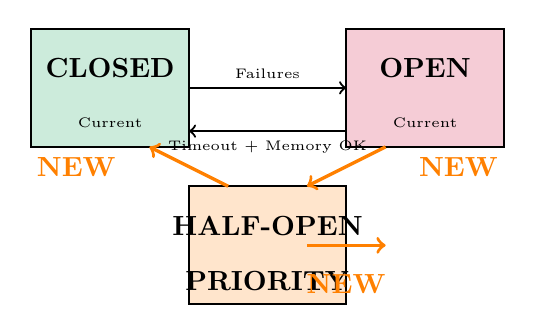
\begin{tikzpicture}[scale=1.0]
            % Current states
            \draw[thick,fill=successgreen!20] (-3,2) rectangle (-1,3.5);
            \node at (-2,3) {\textbf{CLOSED}};
            \node at (-2,2.7) {\circuitclosed};
            \node at (-2,2.3) {\tiny Current};
            
            \draw[thick,fill=alertred!20] (1,2) rectangle (3,3.5);
            \node at (2,3) {\textbf{OPEN}};
            \node at (2,2.7) {\circuitopen};
            \node at (2,2.3) {\tiny Current};
            
            % Future Half-Open State
            \draw[thick,fill=orange!20,thick] (-1,0) rectangle (1,1.5);
            \node at (0,1) {\textbf{HALF-OPEN}};
            \node at (0,0.7) {\circuithalf};
            \node at (0,0.3) {\textbf{PRIORITY}};
            
            % Current transitions
            \draw[thick,->] (-1,2.75) -- (1,2.75);
            \node[above] at (0,2.75) {\tiny Failures};
            
            \draw[thick,->] (1,2.2) -- (-1,2.2);
            \node[below] at (0,2.2) {\tiny Timeout + Memory OK};
            
            % New transitions (planned)
            \draw[thick,->,orange,very thick] (1.5,2) -- (0.5,1.5);
            \node[right,orange] at (1.8,1.75) {\textbf{NEW}};
            
            \draw[thick,->,orange,very thick] (-0.5,1.5) -- (-1.5,2);
            \node[left,orange] at (-1.8,1.75) {\textbf{NEW}};
            
            \draw[thick,->,orange,very thick] (0.5,0.75) -- (1.5,0.75);
            \node[below,orange] at (1,0.5) {\textbf{NEW}};
        \end{tikzpicture}
    \end{center}
    
    \textbf{Half-Open Implementation Plan:}
    \begin{multicols}{2}
        \begin{itemize}
            \item Limited request testing (1-5 requests)
            \item Success/failure tracking
            \item Configurable probe count
            \item Safe transition logic
            \item Backwards compatibility
            \item Gradual rollout strategy
        \end{itemize}
    \end{multicols}
\end{frame}


\section{Q\&A}


\begin{frame}{Additional Resources}
    \textbf{Documentation \& Links:}
    \begin{itemize}
        \item \textbf{Circuit Breaker Pattern:} Martin Fowler's article
        \item \textbf{Netflix Hystrix:} Original implementation reference
        \item \textbf{Our Implementation:} \texttt{https://gitlab.betgenius.net/leandro.leon/go-breaker}
        \item \textbf{TOML Configuration:} Complete examples in repo
    \end{itemize}
    
    \vspace{0.5cm}
    \textbf{Key Papers \& Articles:}
    \begin{itemize}
        \item "Release It!" by Michael Nygard
        \item "Building Microservices" by Sam Newman
        \item "Site Reliability Engineering" by Google
        \item "The Art of Scalability" by Abbott \& Fisher
    \end{itemize}
    
\end{frame}

\begin{frame}{Questions \& Discussion}
    \begin{center}
        \Huge \textbf{Questions?}
        
        \vspace{1cm}
        
        \Large
        \textbf{SMA - Sports Models APIs Team}\\
        \textbf{Genius Sports}
        
        \vspace{0.5cm}
        
        \begin{tikzpicture}
            \node at (0,0) {
\includegraphics[width=4cm]{genius_sports_logo.png}};
        \end{tikzpicture}
        
        \vspace{0.5cm}
        
        \textbf{Thank you for your attention!}
        
        \vspace{0.3cm}
        
        \normalsize
        🔗 \texttt{https://gitlab.betgenius.net/leandro.leon/go-breaker}
    \end{center}
\end{frame}


\end{document}